% !TEX root = ../thesis.tex

\chapter{Neural network training data}
\label{chap:neural-network-data}

Over their relatively brief existance, neural networks have been shown to perform increasingly impressive tasks (e.g.  \cite{openai2019dota}, \cite{openai2023gpt4}, 
and many more). However, they learn by example. The performance of a neural network is directly linked to the input data it receives during training. If the 
training data is not an accurate example of real world information a network later operates on, insight gained from it is at best an approximation, and at worst
completely randomly generated data. 

As such, it is not a question \textit{if} some neural network architecture can learn to identify an extensive air shower from WCD data, but rather which 
implementation, fed with which information, does. For this purpose, this chapter explains the procedure with which training data is generated. As stated above, this
must occur with a focus on being representative of data actually measured in the SD array. The elected approach to create time traces is modularized. The structure
of this chapter reflects this. First, general comments about the characteristics of background data (i.e. the WCD detector response in the absence of an extensive 
air shower) are made in \autoref{sec:background-dataset}. Next, the process to extract signal originating from CRs is detailed in \autoref{sec:signal-dataset}.
Lastly, building the time trace from the aforementioned modules and drawing samples from it for a neural network to train on is done in 
\autoref{sec:sliding-window-analysis}.

\section{Background dataset}
\label{sec:background-dataset}

While a flux of partices causes elevated ADC levels in both the HG and LG channels of a WCD PMT during a shower event, the lack of such a phenomenon does not imply 
the readout information is uniformly flat. Instead, it hovers around the channels' baseline (c.f. \autoref{sec:surface-detector}) with occasional spikes upwards 
due to low-energy particles impinging on the detector. Coupled with electronic noise from the many digital components in the UUB, this constitutes the data that is 
collected inbetween air shower events.

\subsection{Accidental muons}
\label{ssec:accidental-muons}

Most low-energy background particles present in the detector are muons. These are produced in the upper atmosphere during cascading processes analog to 
\autoref{chap:physical-background}. Due to the low primary energy the electromagnetic component of the shower is thermalized before it reaches surface level. The 
muonic component by itself does not contain enough information to enable an accurate reconstruction of primary energy and origin. This fact, coupled with the high
flux of events at lower energies ($\Upphi|_{E=\SI{100}{\giga\electronvolt}} \approx \SI[per-mode=power]{1}{\per\meter\per\second}$ \cite{boezio2000measurement}) 
make these events unsuitable for analysis. Stray muons, even though they originate from extensive air showers, must consequently be considered background events.

The rate at which such particles traverse a WCD tank is $f_\text{Acc.}\approx\SI{4.665}{\kilo\hertz}$ \cite{DavidInjectionFrequency}. Their arrival time is 
Poisson-distributed. This implies that generally, one in 14 time traces contains signal from a low-energy background event. Coincidences of two accidental 
muons occur on a sub-percent level. Any higher order of coincidences is likely originating from a single air shower process. The typical signal recorded by the 
surface detector from a single muon is presented in \autoref{fig:muon-response}

\begin{figure}
	\centering
	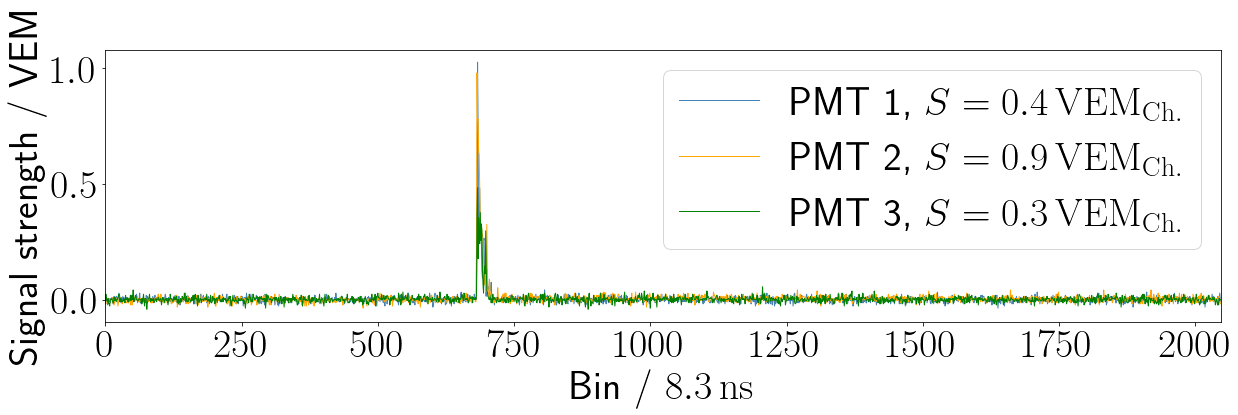
\includegraphics[width=0.8\textwidth]{./plots/muon_response.png}
	\caption{The simulated time trace from a single muon. The maximum peak of the time trace is equal \SI{1}{\Peak}. The integrated signal $S$ is of comparable
	magnitude.}
	\label{fig:muon-response}
\end{figure}

\subsection{Electronic noise}
\label{ssec:electronic-noise}

Electronic noise is the umbrella term given to the distortions that some signal is subject to during digital readout. Such noise can have many different origins.
An illustrative example is given by the \textbf{L}aser \textbf{I}nterferometer \textbf{G}ravitational wave \textbf{O}bservatory, which excludes the \SI{60}{\hertz}
band and its' harmonics from analysis. This is owed to the fact that the DC frequency standard in the United States introduces systematic uncertainties in the
detector \cite{martynov2016sensitivity}. In the electronics of Pierre Augers' SD array, electronic noise is assumed to be Gaussian. That is to say that the 
\SI{}{\ADC} values of a time trace that was measured while no particle produced signal in the tank are normally distributed around the baseline. The standard 
deviation can be estimated from monitoring data, as is shown in \autoref{fig:standard-deviation-baseline}. \todo{make this plot}

\begin{figure}
	\centering
	\includegraphics[width=0.8\textwidth]{./plots/standard_deviation_baseline.png}
	\caption{Example variance of all UUB stations in the surface detector array. The data shown in this plot was recorded on November 15th 2022 and is collected 
	regularly via monitoring processes. }
	\label{fig:standard-deviation-baseline}
\end{figure}

\subsection{Random traces}
\label{ssec:random-traces}

Both above mentioned phenomena can be simulated, and the simulation results used as background training data for the neural networks discussed in the next chapter.
A more accurate method however, and the approach elected for this work is to utilize directly measured data from the field. Thanks to the work of David Nitz, there 
exist collections of so called random traces that were gathered by forcing DAQ readout via a manually set trigger. 

In particular, two datasets of UUB random traces have been created until now. They were taken from 13th-18th March 2022, and 14th-18th November 2022 respectively. 
The first set contains data a total of sixteen million time traces distributed over four different SD stations. For reasons explained in 
\autoref{ssec:random-trace-calibration}, only data from the first set is used in the analysis presented in this work.

\subsubsection{Characteristics}
\label{ssec:random-trace-characteristics}

Contrary to the naming of the random trigger, it occurs at a deterministic time. More accurately, the process of measuring random traces is as follows;
A single time trace ($2048\cdot\SI{8.333}{\nano\second} = \SI{17.07}{\micro\second}$) is written to the local station buffer every $\SI{10}{\milli\second}$. Once
the buffer has accumulated enough data, it is written to a USB storage device. Because of a bottleneck in the last step, the process takes about \SI{22}{\hour}
per station \cite{nitzCorrespondence}.

It is thus not the trigger that is unpredictable, but the data measured by each trigger. Due to the read/write process being indepentant of the measured data
(as opposed to the algorithms in \autoref{chap:classical-triggers}) the latter must be considered to be essentially random. For the most part, random traces are 
assumed to consist solely of electronic noise. However, signal of cosmic origin - be it accidental muons or extensive air showers - will appear in the data at a
rate at least consistent with \autoref{sec:classical-triggers-performance}.

A crude analysis of the type of noise in the random traces can be made by examining the spectral density of the dataset, shown in \autoref{fig:random-traces}.
Harmonic modulations visible in both spectra might originate from an offset between last and first bin of the random traces. If this offset is nonzero, the 
periodic extension of $f(x)$ exerts a step-function-like behaviour. The Fourier transform consequently reflects this \cite{burrows1990fourier}. Still, several
features of $| \hat{f}(\xi) | ^{2}$, espically present at $\SI{10}{\mega\hertz}$, imply the presence of systematic noise in the UUB. Nevertheless, the large scale 
form of the spectral density is compatible with at least two noise models, that cannot be distinguished based on the data at hand:

\begin{itemize}
	\item  $\mathbf{| \hat{f}(\xi) | ^{2} \propto \exp\left(\frac{(\xi - \mu)^2}{2\sigma^2}\right)}$. The spectral density is Gaussian. This implies the noise is 
	Gaussian distributed as well, confirming the assumption in \autoref{ssec:electronic-noise}.
	\item $\mathbf{| \hat{f}(\xi) | ^{2} \propto} \exp\left(-m\xi + b\right)$. The spectral density is proportional to $\xi^{-n}$ for some power $n$. The case $n = 2$
	($\SI[per-mode=symbol]{-6}{\deci\bel\per\octave}$ attenuation) seems to describe the observations well, hinting that the generating function could be Brownian.

\end{itemize}

\begin{figure}
	\centering
	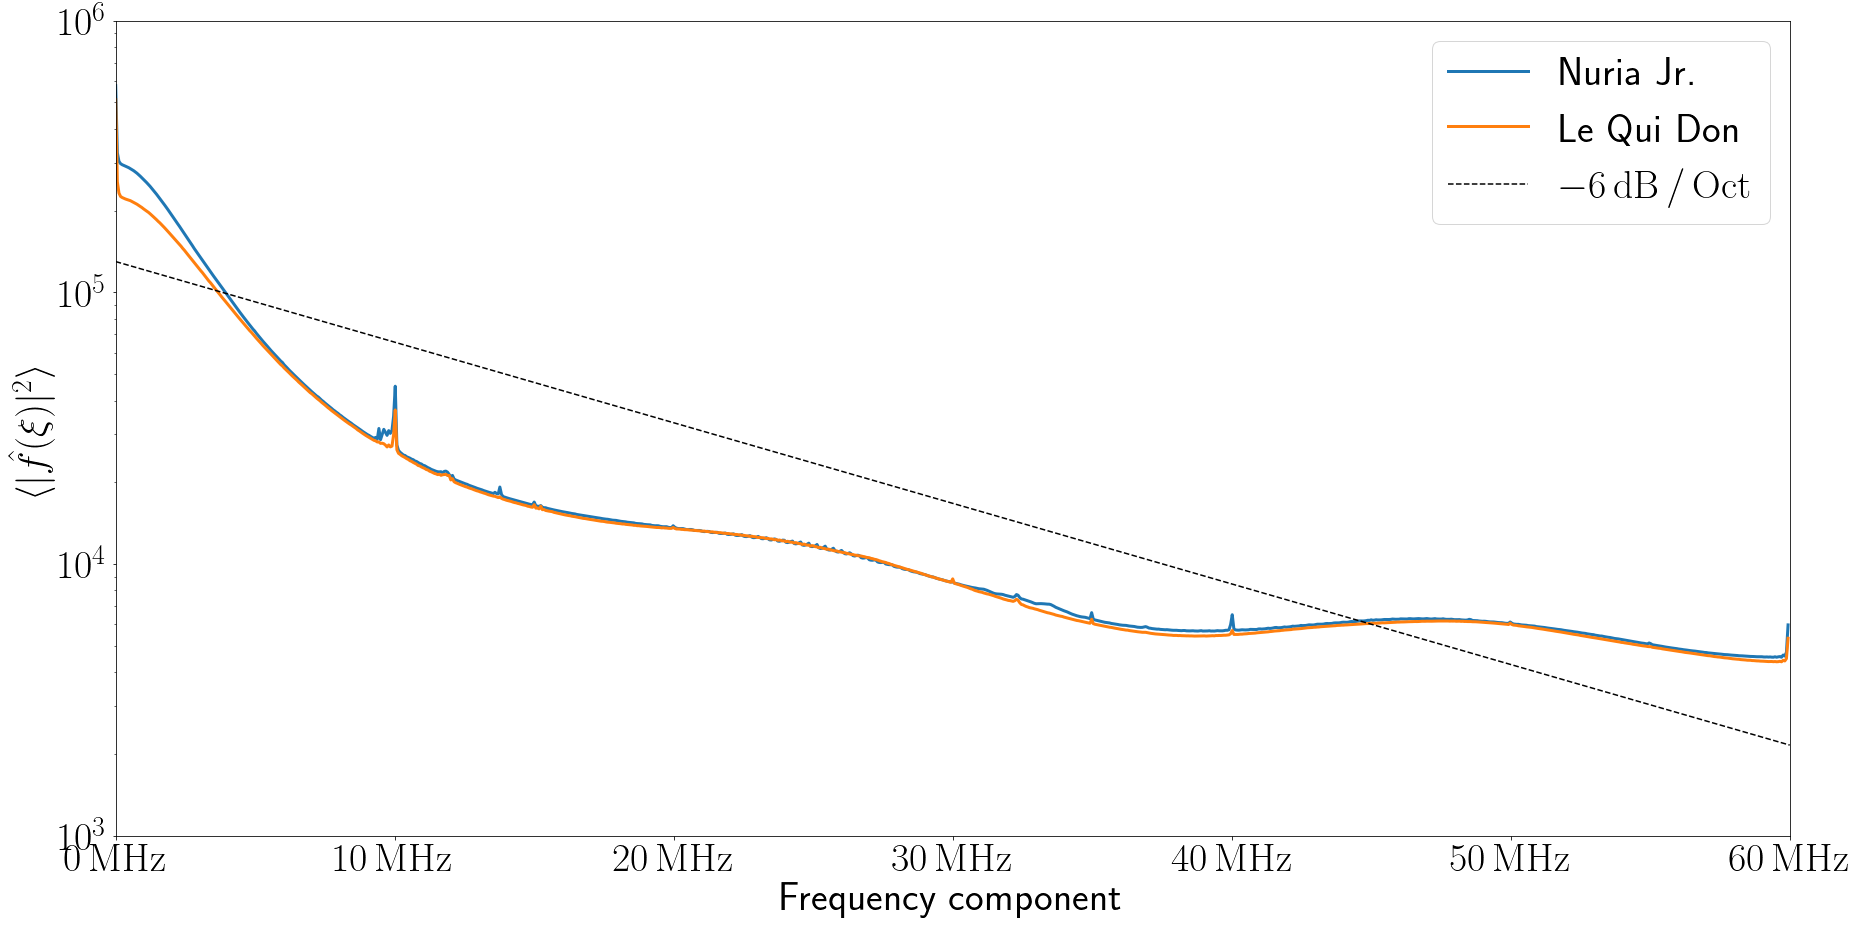
\includegraphics[width=0.8\textwidth]{./plots/random_trace_spectral_density.png}
	\caption{The random trace spectral density for two stations. Plotted with a dashed black line is reference attenuation curve falling at 
	$\SI[per-mode=symbol]{-6}{\deci\bel\per\octave}$. The spike at \SI{10}{\mega\hertz} is of unknown origin and represents systematic noise in the UUB 
	electronics.}
	\label{fig:random-traces}
\end{figure}

\subsubsection{Calibration}
\label{ssec:random-trace-calibration}

The random trace files contain raw measurement data in units of $\SI{}{\ADC}$ for the HG and LG channel of the three WCD PMTs. In a first step to standardize this
information, the baseline is substracted from each FADC bin. This is done via the baseline finding algorithm described in \autoref{ssec:offline-calibration} and 
\cite{tobiasBaseline, tobiasBaselineUUB}. Note that this approach differs from the baseline finding algorithm that runs on each station (c.f. 
\autoref{ssec:online-calibration}). However, the difference is negligible ($<<\,\SI{1}{\ADC}$) for traces that do not contain any signal, which is the case for the 
vast majority of the dataset.

Next, the baseline-substracted time traces are converted from units of $\SI{}{\ADC}$ to $\SI{}{\Peak}$. This conversion is not straight forward however, as it 
requires knowledge of \Ipeak at the time of data taking. Each station estimates this value in periodic time intervals in the context of monitoring diagnostics.

For the second dataset of random traces (taken from 14th-18th November 2022) a UNIX timestamp packaged with each time trace may be related to monitoring data. This 
reveals that no information regarding \Ipeak was forwarded to CDAS for any station while it recorded random traces. This unfortunately renders the entire dataset 
useless in the context of this work.

For the first collection of random traces, monitoring data is available, but there exists no timing information for the individual traces. The elected procedure to 
evaluate data as accurately as possible is thus to calculate the day average of \Ipeak and \Qpeak

\todo{procedure}
\todo{rate mismatch}

\section{Signal dataset}
\label{sec:signal-dataset}



\section{Trace building \& Sliding window analysis}
\label{sec:sliding-window-analysis}
